% Не забудьте установить пакет cm-super
%   для использования векторных шрифтов при генерации документа
\documentclass[fleqn, xcolor=x11names]{beamer}

\usepackage{pgfplots}
\pgfplotsset{compat=1.18}
\usetheme{MyAmsterdam} % тема
\usecolortheme{default}

\usepackage[T2A]{fontenc}
\usepackage[utf8x]{inputenc}
\usepackage[english,russian]{babel}
\usepackage{amsmath}
\usepackage{amsfonts}
\usepackage{amssymb}
\usepackage{hyperref}
\usepackage{graphics, graphicx}
\usepackage{color}
\usepackage{enumerate}

\usepackage{pgfplots}
\usetikzlibrary{patterns}

\usepackage{minted}
\usemintedstyle{default}

\usefonttheme[onlymath]{serif}  % привычный шрифт для математических формул
\usepackage[nopar]{lipsum} %для генерации большого текста

\definecolor{bg}{rgb}{0.95,0.95,0.95}

\usepackage{tcolorbox}

\newcommand{\real}{\mathbb{R}}
\newcommand{\norm}{\mathop{\rm norm}\limits}
\newcommand{\softmax}{\mathop{\rm softmax}\limits}

\definecolor{beamer@blendedblue}{rgb}{0.037,0.366,0.75}
\defbeamertemplate{footline}{myframe number}
{
  \hfill%
  \usebeamercolor[fg]{page number in head/foot}%
  \usebeamerfont{page number in head/foot}%
  \raisebox{5pt}[0pt][0pt]{% <--- change here
    \insertframenumber\,/\,\inserttotalframenumber\kern1em}%
}
\setbeamertemplate{footline}[myframe number]

\title[Введение в Python]{\bfseries Занятие 5.1: Написание текстовых отчётов и научных текстов}
\author[Находнов~М.\,С.]{Находнов Максим Сергеевич}
\subtitle{Практикум на ЭВМ, осень 2022}
\institute[OM]{кафедра ММП, ВМК МГУ}
\date{06 октября 2022 г.}

\graphicspath{{Figures/}} % относительный путь к каталогу с рисунками - чтобы каждый раз не писать

\begin{document}

\begin{frame}
    \maketitle
\end{frame}

\begin{frame}{Написание научных текстов}

\textsl{Научные тексты:} научные статьи, отчеты, курсовые, выпускные работы и т.д.

\hfill

Есть правила (стандарты) написания научных текстов.

\hfill

\textbf{Зачем нужны правила?}

Чтобы разные люди без дополнительных усилий понимали друг друга. Чем жёстче требования к терминологии, языку, форме подаче материала, оформлению, тем быстрее читатель сможет понять основную суть работы.

\hfill

На этой паре разбираем, как писать отчёты.
\end{frame}

\begin{section}{Составление отчёта}

\begin{frame}[fragile]\frametitle{Типичная структура отчёта}
	Структура отчёта примерно соответствует пунктам задания:

	\begin{enumerate}
		\item \textbf{Титульная страница} (Заголовок)
		\item (опционально) \textbf{Оглавление}
		\item Введение
		\item (опционально) \textbf{Пояснения к задаче}, например, выкладки для основных формул в работе
		\item \textbf{Список экспериментов}
		\begin{enumerate}
			\item Дизайн эксперимента
			\item Результаты эксперимента
			\item Выводы из эксперимента
		\end{enumerate}
		\item \textbf{Общие выводы} из работы
		\item (опционально) \textbf{Список использованной литературы}
		\item (опционально) \textbf{Аппендиксы}, например, вспомогательные выкладки, пояснения
	\end{enumerate}

\end{frame}

\begin{frame}[fragile]\frametitle{У отчёта должен быть \textbf{заголовок}}
Из заголовка должно быть понятно:
\begin{itemize}
    \item Кем выполнено задание?
    \item Какое задание выполнено?
    \item К какому курсу относится задание?
\end{itemize}

\hfill

Необязательно верстать титульную страницу!

\hfill


\end{frame}

\begin{frame}[fragile]\frametitle{У отчёта должно быть \textbf{введение}}
Из введения должно быть понятно:
\begin{itemize}
    \item В чём заключалось задание?
\end{itemize}

\hfill

Введение не повторяет полностью формулировку задания, а лишь кратко описывает её.

Можно ссылаться на формулировку задания, если не получается кратко сформулировать все аспекты.

\hfill

Введение должно быть конкретным (относится к конкретному заданию, а не к выбранной области анализа данных в целом).
\end{frame}

\begin{frame}[fragile]\frametitle{Пример неконкретного введения к заданию}
Компьютеры все чаще и чаще выступают помощниками человека. Водитель, потеряв дорогу, скорее воспользуется навигатором, чем спросит путь
у прохожего или другого водителя. Захотев связаться с кем-то, мы скорее
напишем ему письмо, состоящее из байтов, чем из бумаги и чернил. То же
самое можно сказать и о распознавании изображений. Возьмем, как пример,
ЕГЭ. Множество учеников со всей России заполняют огромное количество
бланков, и все эти бланки необходимо проверить. Что же делать в этой
ситуации? Ведь вряд ли кто согласится проверять эти бланки. И здесь на
помощь приходят компьютеры. Они распознают ответы учеников и заполняют по ним базу данных, откуда берутся данные для подсчета результата экзамена. Теме анализа изображения, а точнее, анализа рукописного текста, и посвящена данная работа.
\end{frame}

\begin{frame}{\textbf{Описание экспериментов}: как не надо делать}
\begin{center}
    \fbox{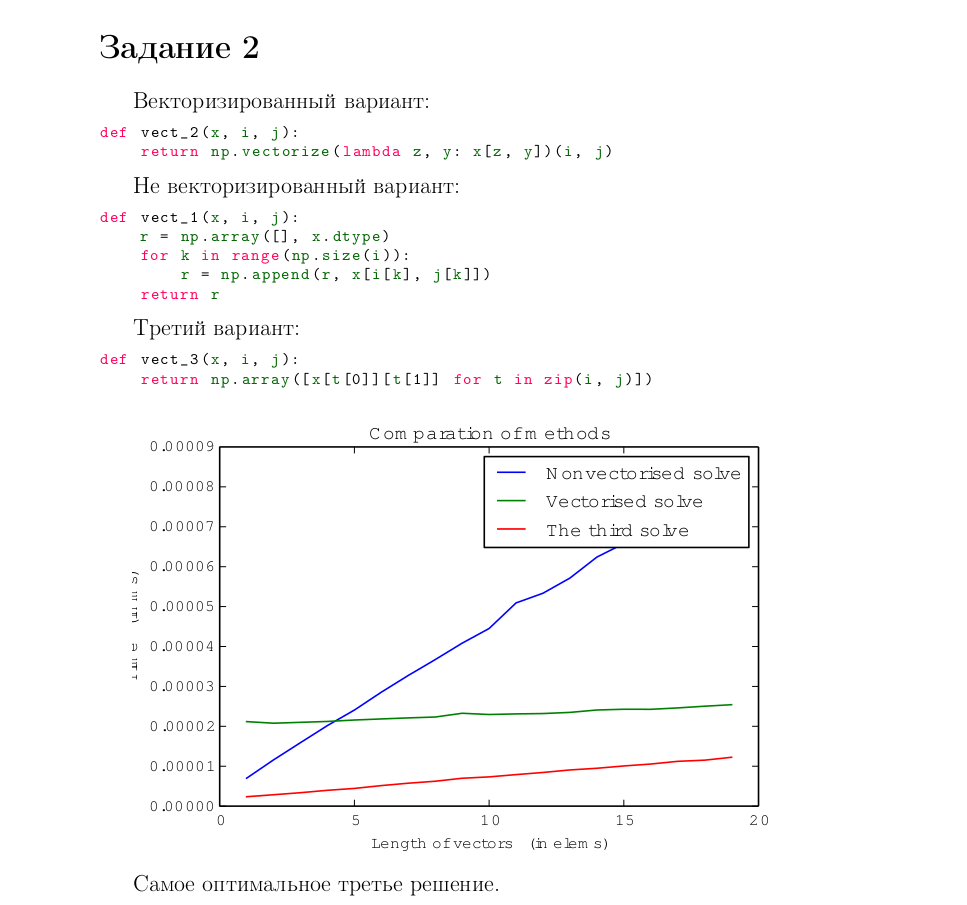
\includegraphics[height=6.5cm]{no_reason.png}}
\end{center}
Эксперименты не описаны, нет выводов.
\end{frame}

\begin{frame}{\textbf{Описание экспериментов}: как  надо делать}
\begin{center}
\fbox{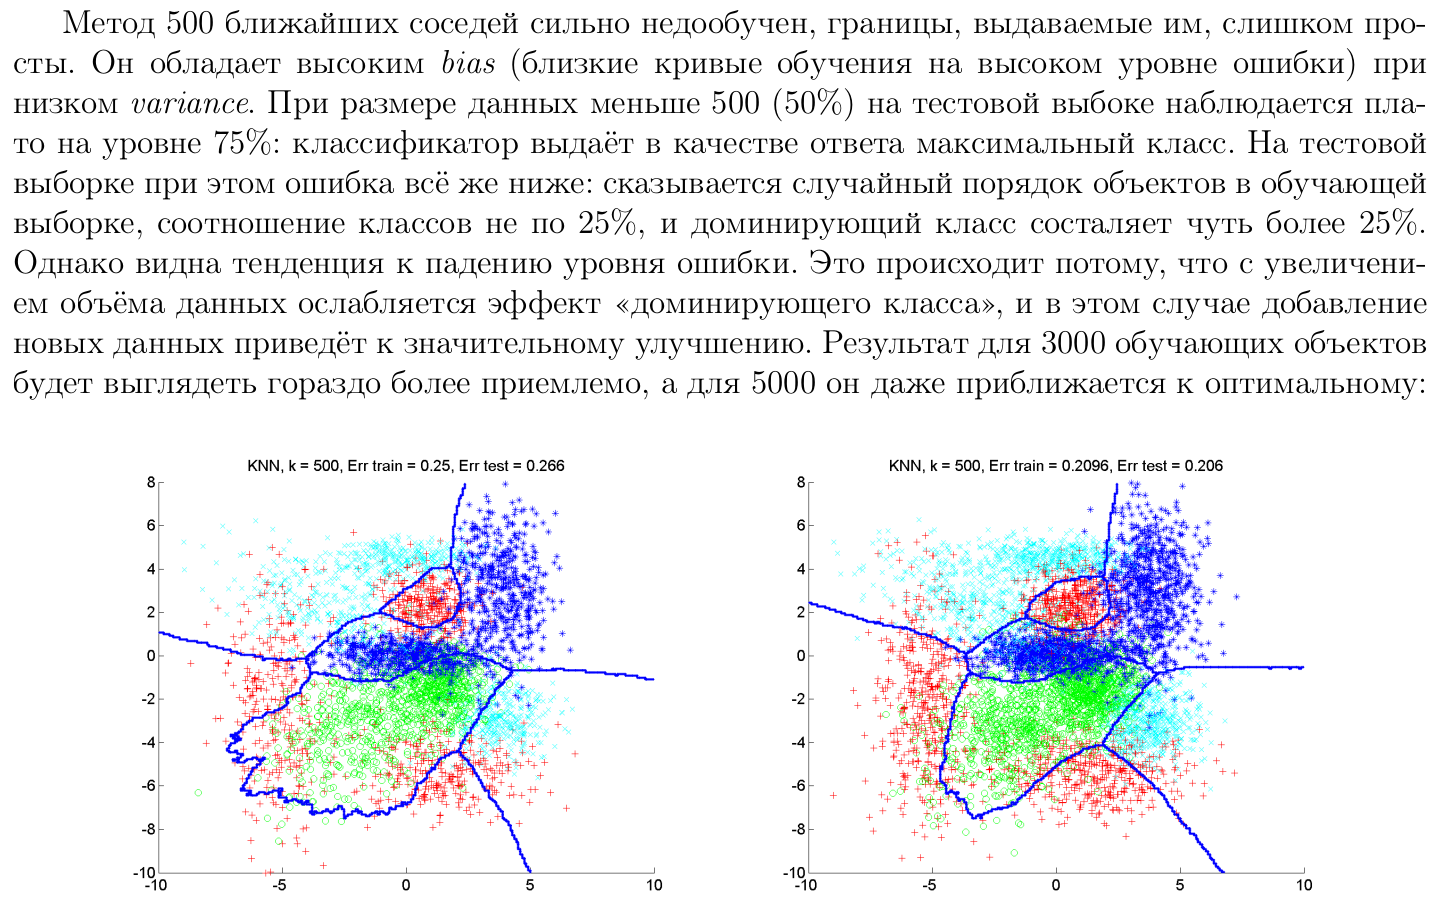
\includegraphics[height=6.5cm]{good_reason.png}}
\end{center}
Проведён анализ и на его основе сделаны выводы.
\end{frame}

\begin{frame}{Анализируйте результаты экспериментов}
\begin{table}[]
    \begin{tabular}{|c|c|c|c|}
        \hline
        размер данных & numpy & only python & смешанная \\ \hline
        $10$                                      & $1.2$   & $50.21$      & $2.1$       \\ \hline
        $100$                                     & $2.52$  & $40.1$       & $10.2$      \\ \hline
        $1000$                                    & $4.5$   & $45.34$      & $30.95$     \\ \hline
    \end{tabular}
\end{table}

\hfill

\textcolor{red}{Что в этих результатах подозрительно?}

\hfill
\pause{
    \begin{itemize}
        \item Вычисления для размерности $100$ и $1000$ происходит быстрее чем для $10$.
    \end{itemize}
}
\end{frame}

\begin{frame}{Используйте векторные шрифты}
\tabcolsep=10pt
\begin{tabular}{ll}
    Растровые шрифты: & Векторные шрифты: \\
    
\includegraphics[width=4.5cm]{bitmap_fonts.pdf} & 
\includegraphics[width=4.5cm]{vector_fonts.pdf}
\end{tabular}

\

Для генерации текстов с векторными шрифтами достаточно установить пакет \TeX\ \texttt{cm-super}.
\end{frame}

\end{section}

\begin{section}{Оформление графиков}

\begin{frame}{Оформление графиков. Некоторые советы}
    Графики должны быть с одной стороны понятными и информативными, а с другой стороны \textit{красивыми}.

	\begin{center}
		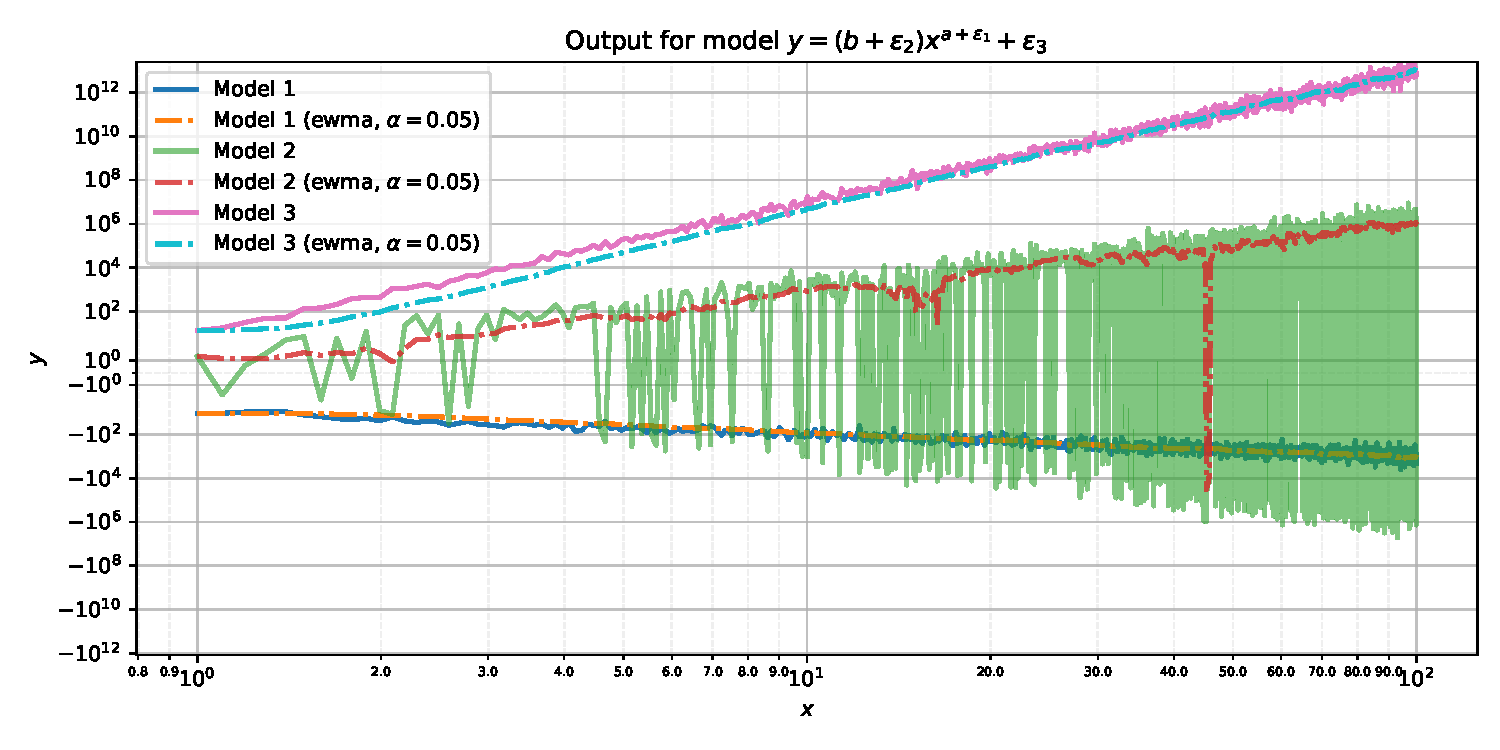
\includegraphics[height=5.5cm]{bad_plots/good_plot.pdf}
	\end{center}
\end{frame}

\begin{frame}{Используйте векторную графику}
    \begin{itemize}
        \item Все графики должны быть отрисованы в векторном формате
    \end{itemize}

	\begin{center}
		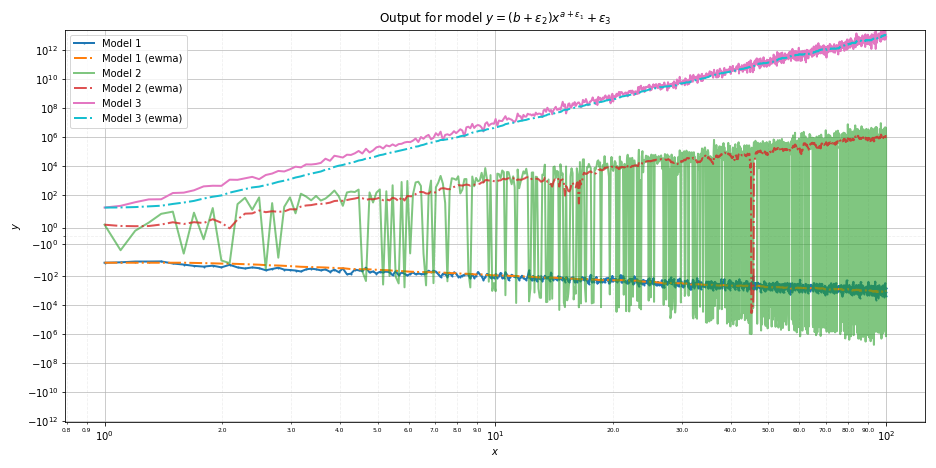
\includegraphics[height=5.5cm]{bad_plots/non_vector_plot.png}
	\end{center}
\end{frame}

\begin{frame}{Рисуйте сетку на графиках}
    \begin{itemize}
        \item На всех графиках без исключения должна быть нарисована сетка
    \end{itemize}

	\begin{center}
		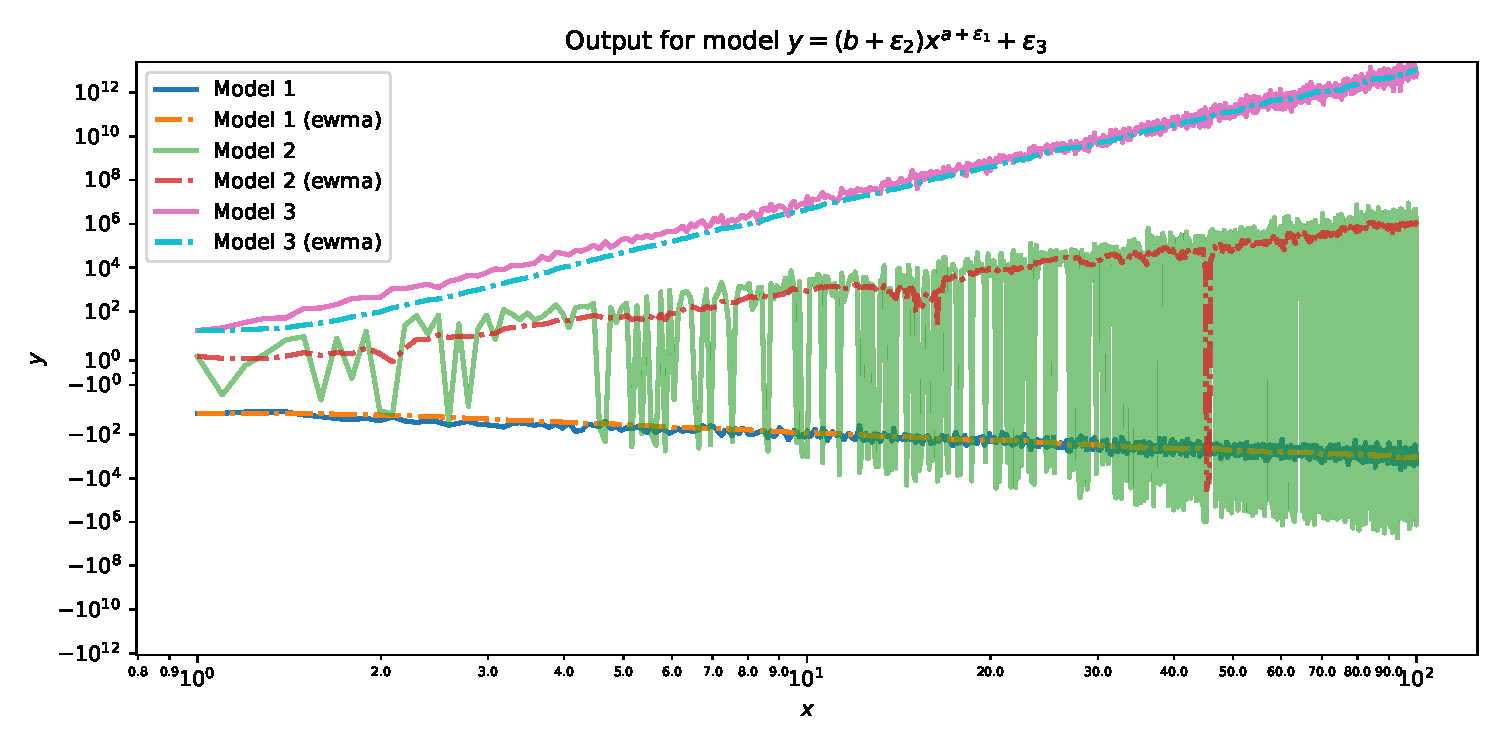
\includegraphics[height=5.5cm]{bad_plots/no_grid_plot.pdf}
	\end{center}
\end{frame}

\begin{frame}{Подписывайте все части графика}
    \begin{itemize}
        \item Все графики и группы графиков должны иметь заголовок
        \item При необходимости оси должны быть подписаны
        \item Если на графике отображено несколько сущностей, то необходима исчерпывающая легенда
    \end{itemize}

	\begin{center}
		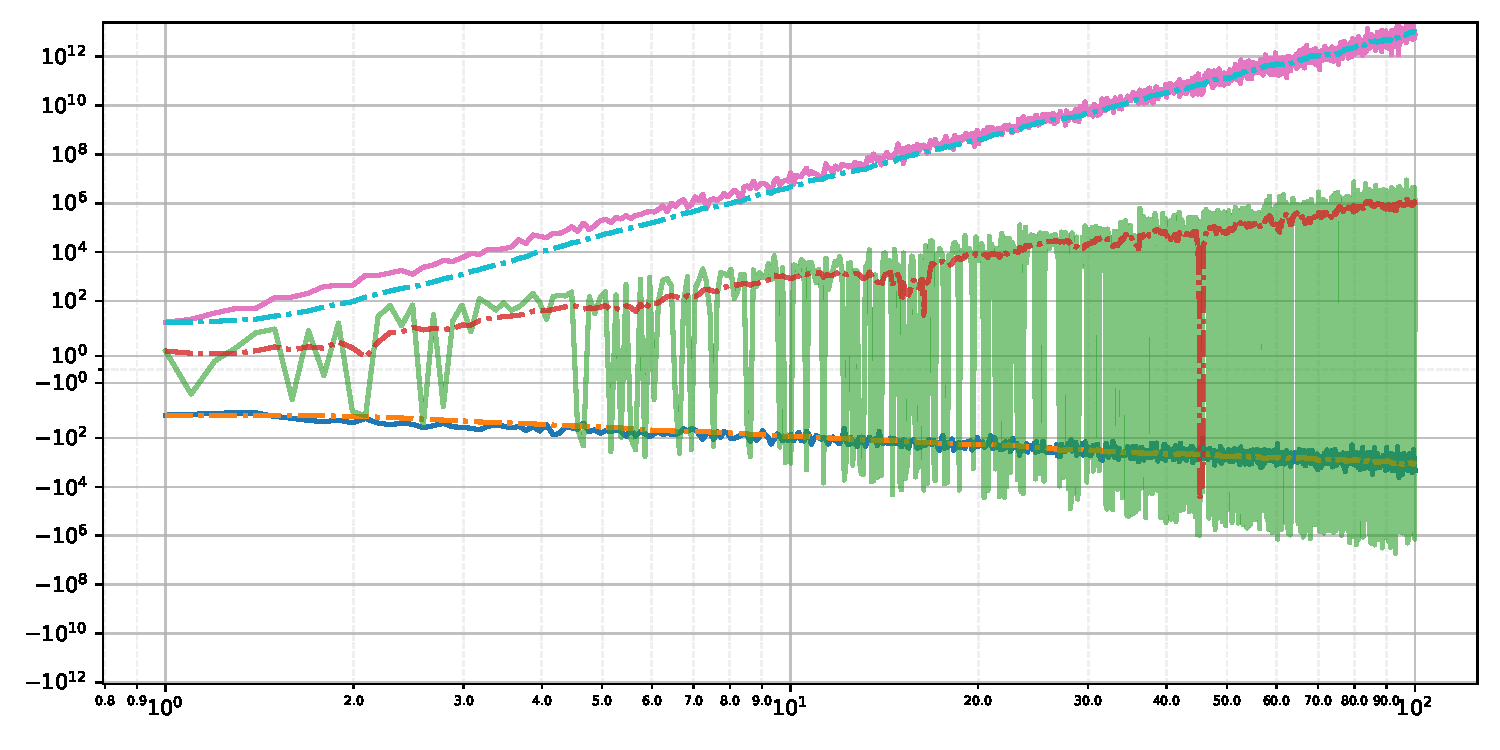
\includegraphics[height=5.3cm]{bad_plots/no_labels_plot.pdf}
	\end{center}
\end{frame}

\begin{frame}{Выбирайте правильные стили}
    \begin{itemize}
        \item Все линии на графиках должны быть чётко видны
        \item Используйте \textit{красивую} цветовую палитру с хорошо различимыми цветами
    \end{itemize}

	\begin{center}
		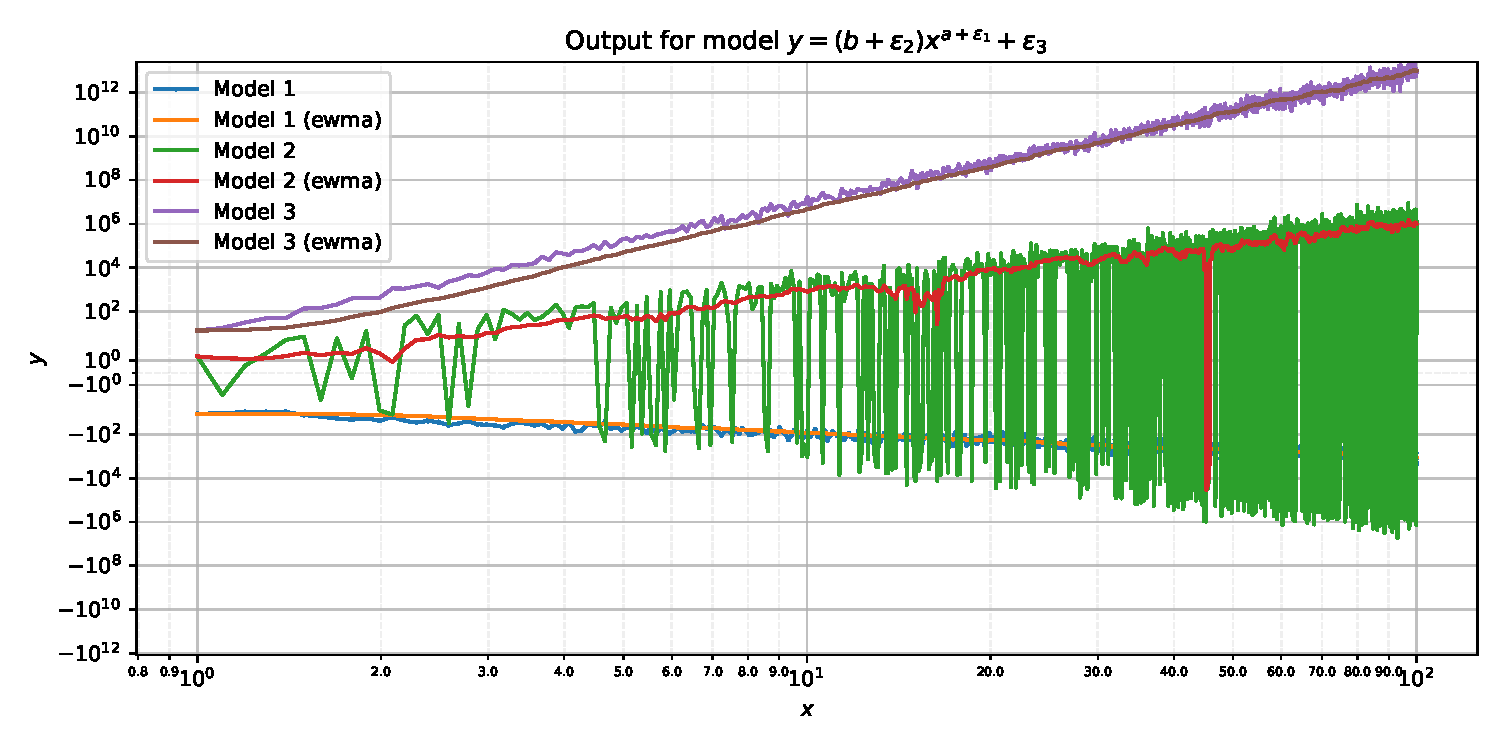
\includegraphics[height=5.5cm]{bad_plots/non_optimal_style_plot.pdf}
	\end{center}
\end{frame}

\begin{frame}{Используйте правильный масштаб}
    \begin{itemize}
        \item Масштаб по каждой оси на графике должен быть выбран правильно
    \end{itemize}

	\begin{center}
		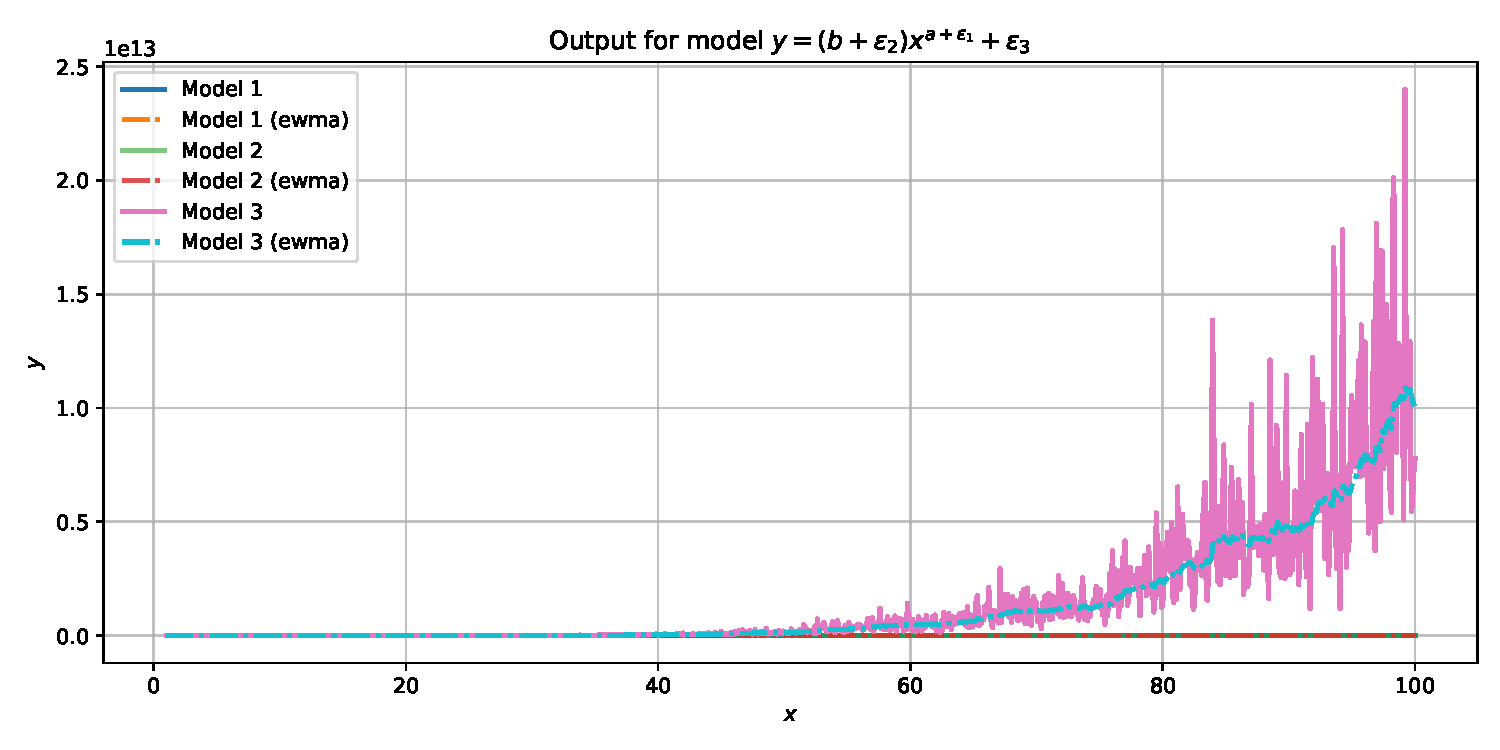
\includegraphics[height=5.5cm]{bad_plots/no_scaling_plot.pdf}
	\end{center}
\end{frame}

\begin{frame}{Используйте \LaTeX}
    \begin{itemize}
        \item Написания формул в заголовках, легенде и в подписях осей необходимо выполнять с помощью \LaTeX
    \end{itemize}

	\begin{center}
		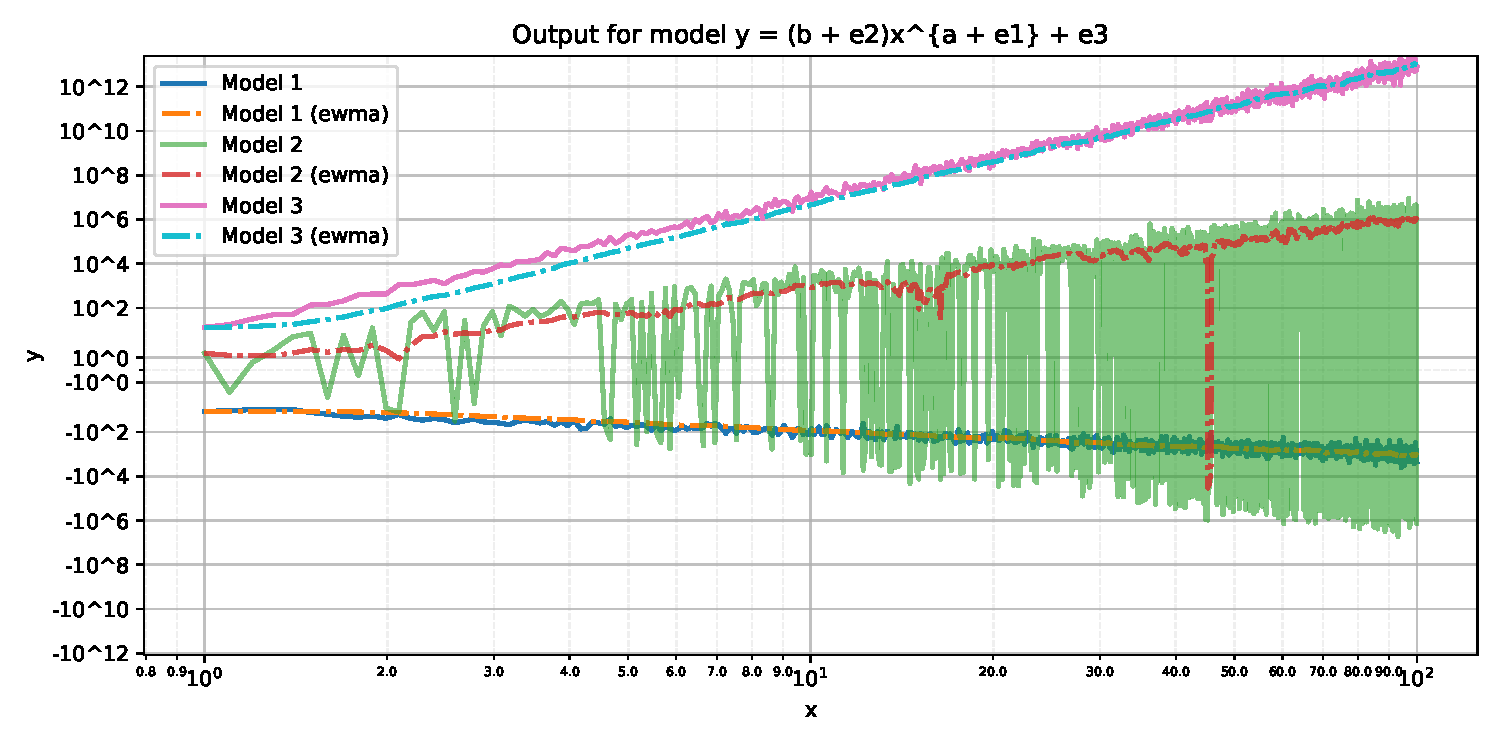
\includegraphics[height=5.5cm]{bad_plots/no_latex_plot.pdf}
	\end{center}
\end{frame}

\begin{frame}{Подбирайте адекватный размер графика}
    \begin{itemize}
        \item Графики должны быть не супер-микро и не супер-макро по размерам, так, чтобы можно было увидеть все, что нужно
    \end{itemize}

	\begin{center}
		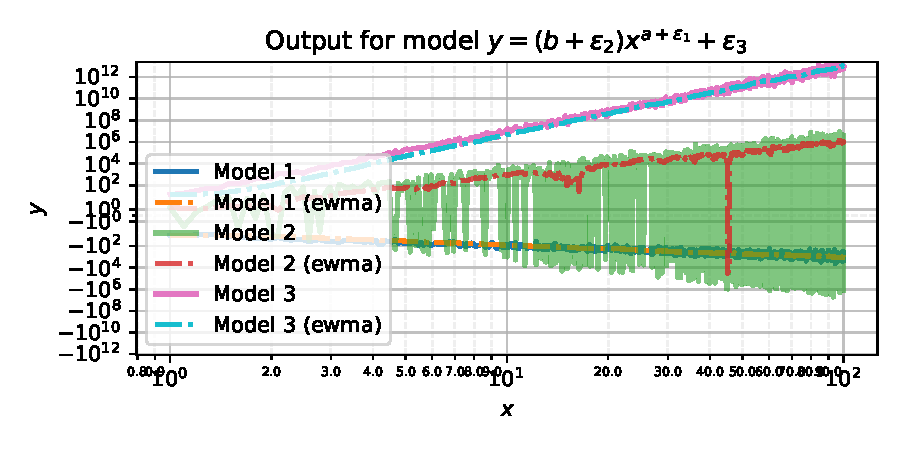
\includegraphics[height=3.5cm]{bad_plots/no_resize_plot.pdf}
	\end{center}
\end{frame}

\begin{frame}{Пример плохого графика из жизни}
	\begin{center}
		\fbox{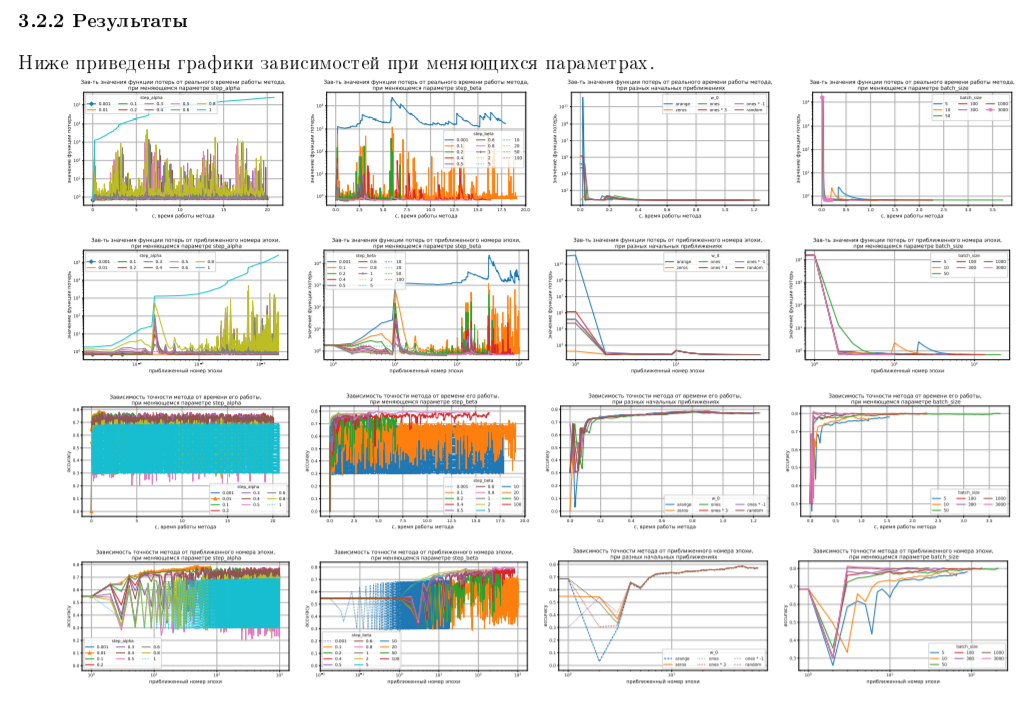
\includegraphics[height=6.5cm]{small_plots.png}}
	\end{center}
    \pause{Много подробных графиков, но все они нечитаемы!}
\end{frame}

\begin{frame}{Пример плохого графика из жизни}
	\begin{center}
		\fbox{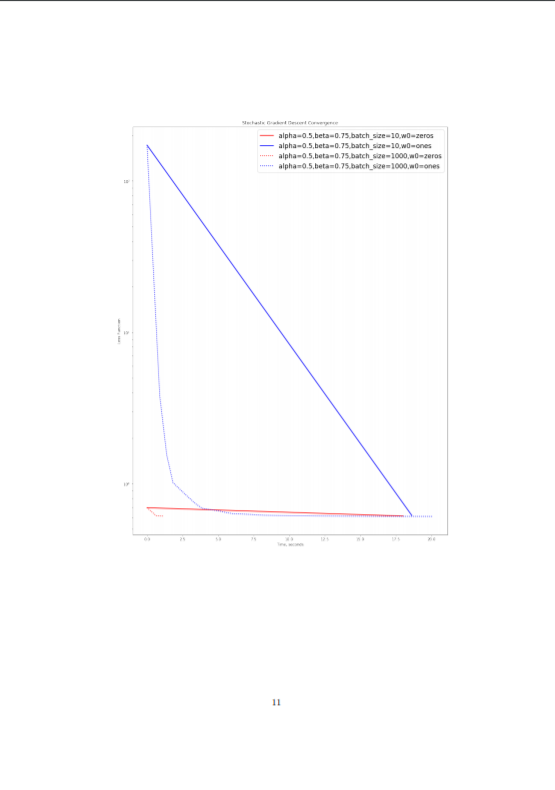
\includegraphics[height=6cm]{huge_plots.png}}
	\end{center}
	\pause{Тут --- наоборот, большой график. Однако понять, что на нём происходит, нельзя.}
\end{frame}

\begin{frame}{Пример плохого графика из жизни}
	\begin{center}
		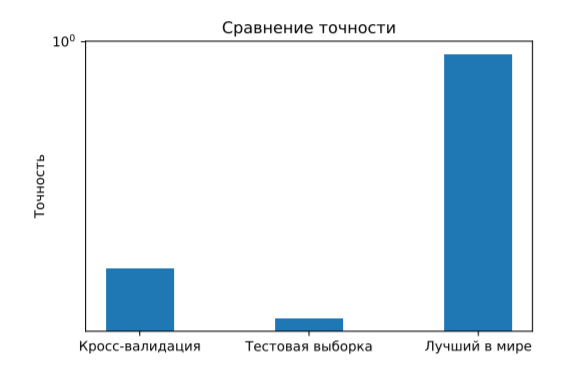
\includegraphics[height=6.5cm]{missing_ticks.png}
	\end{center}
	\pause{Плохо подобраны отсчёты на вертикальной шкале.}
\end{frame}

\begin{frame}{Пример плохого графика из жизни}
	\begin{center}
		\fbox{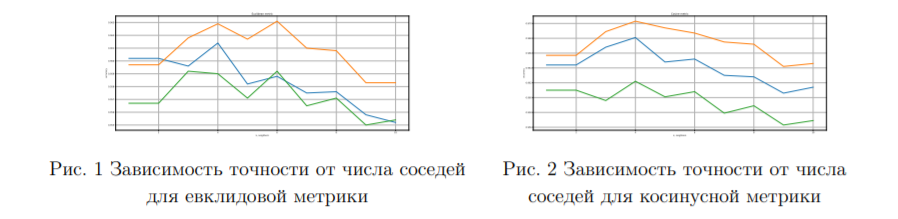
\includegraphics[height=2.5cm]{extra_small_ticks.png}}
	\end{center}
	\pause{Отсчёты не видно.}
\end{frame}

\begin{frame}{Пример плохого графика из жизни}
    \begin{center}
        \fbox{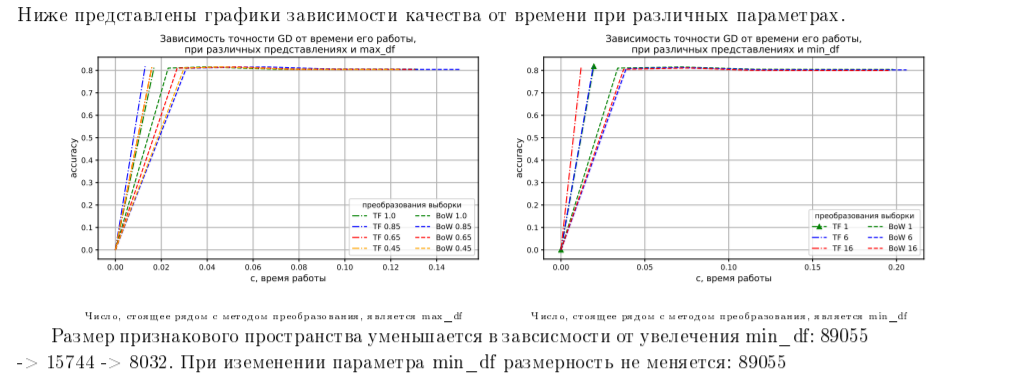
\includegraphics[height=4.0cm]{small_ticks.png}}
    \end{center}
    \pause{Подпись графика слишком мелкая.}
\end{frame}

\begin{frame}{Примеры графиков из жизни}
\begin{center}
    \tabcolsep=15pt
    \begin{tabular}{ll}
        Плохой график: & Хороший график: \\
        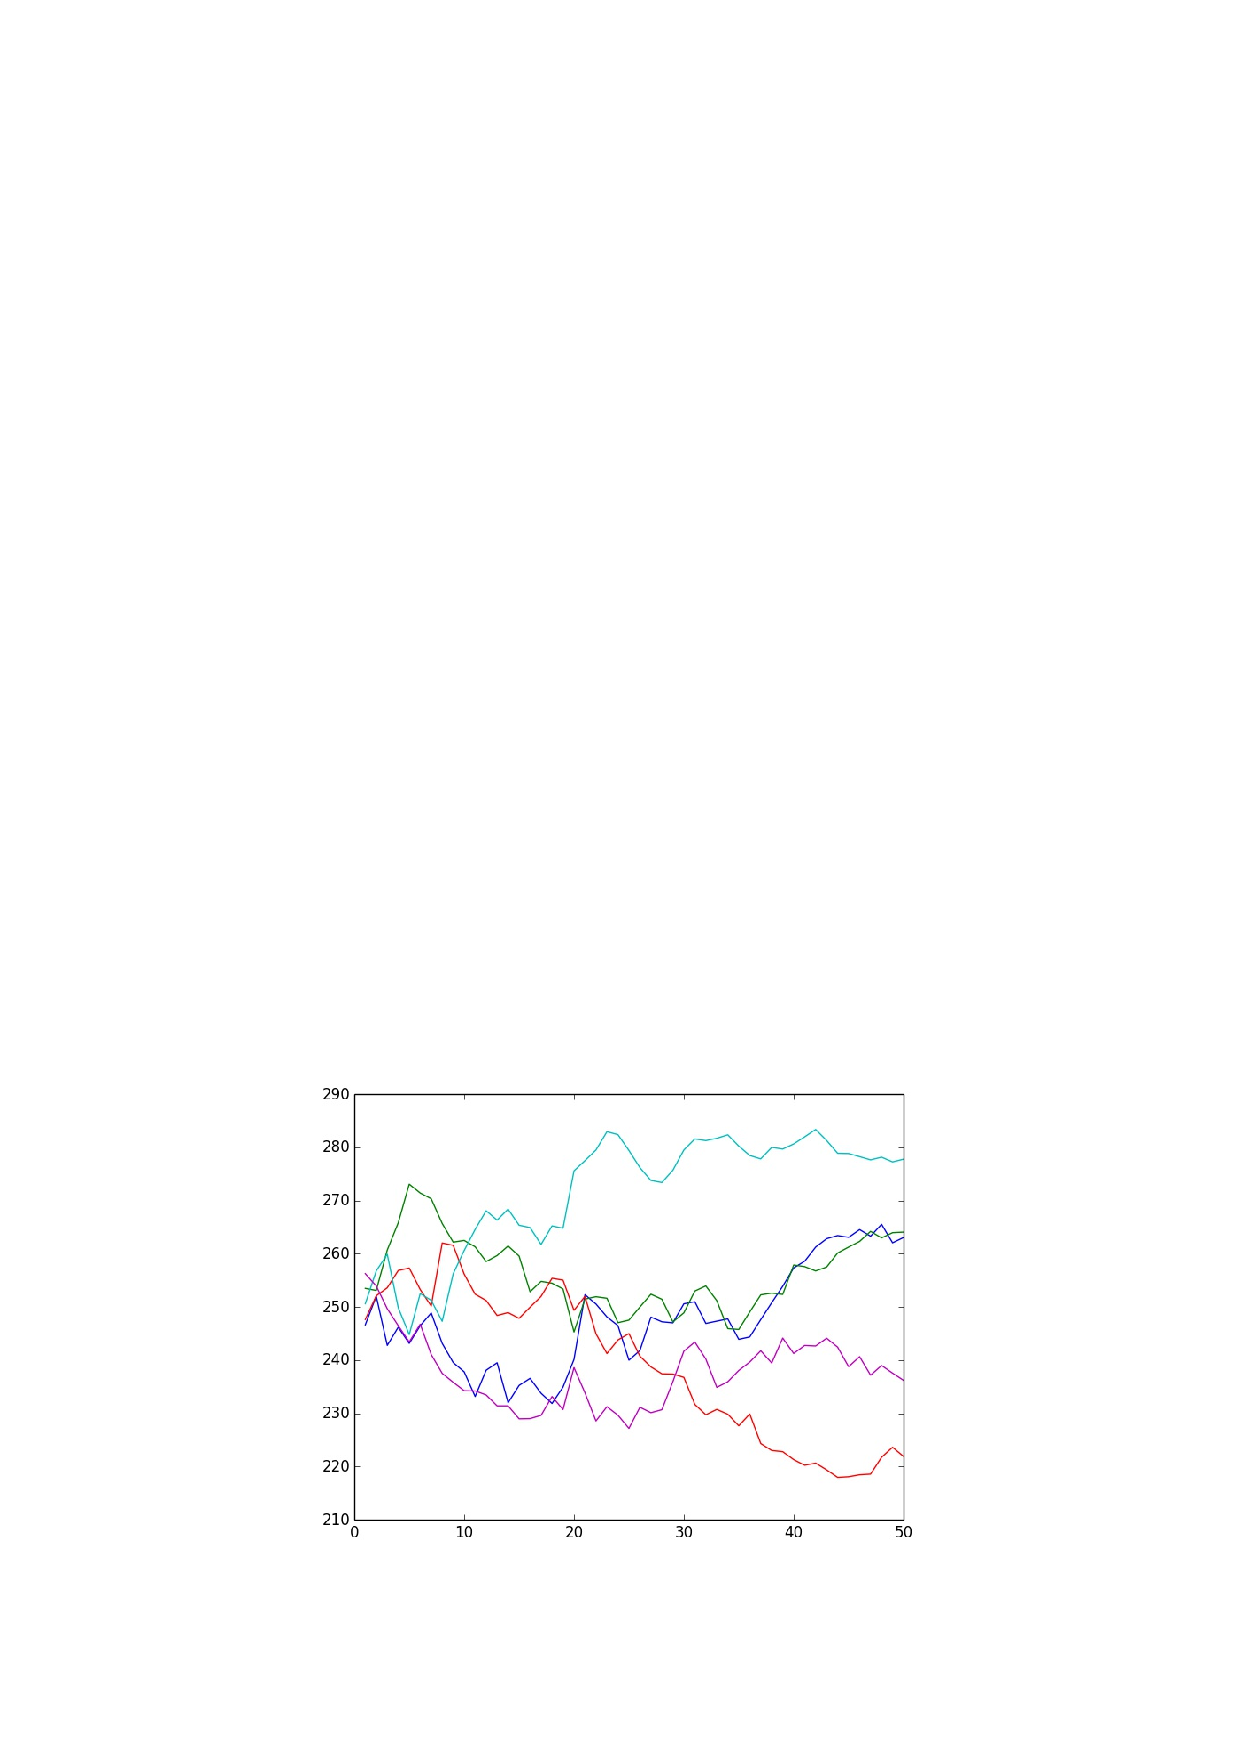
\includegraphics[height=3.5cm]{bag_picture.pdf} & 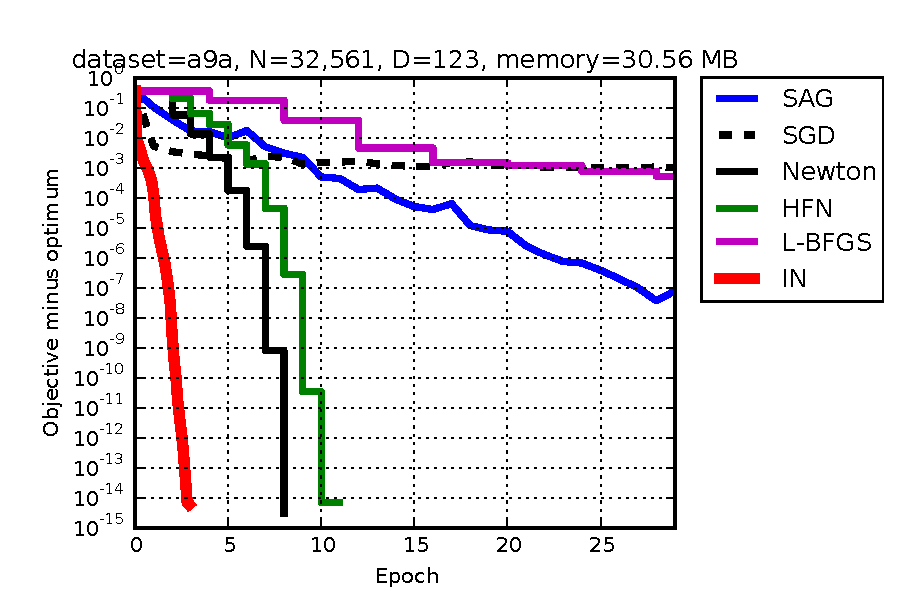
\includegraphics[height=3.5cm]{a9a_epoch.pdf}
    \end{tabular}
\end{center}

Элементы хорошего графика:
\begin{itemize}
    \item Все линии жирные;
    \item Есть легенда;
    \item По осям указаны значения, сами оси подписаны;
    \item По осям выбрана правильная шкала;
    \item Сохранён в векторном формате.
\end{itemize}

\end{frame}

\begin{frame}{Пример хорошего графика из жизни}
	\begin{center}
		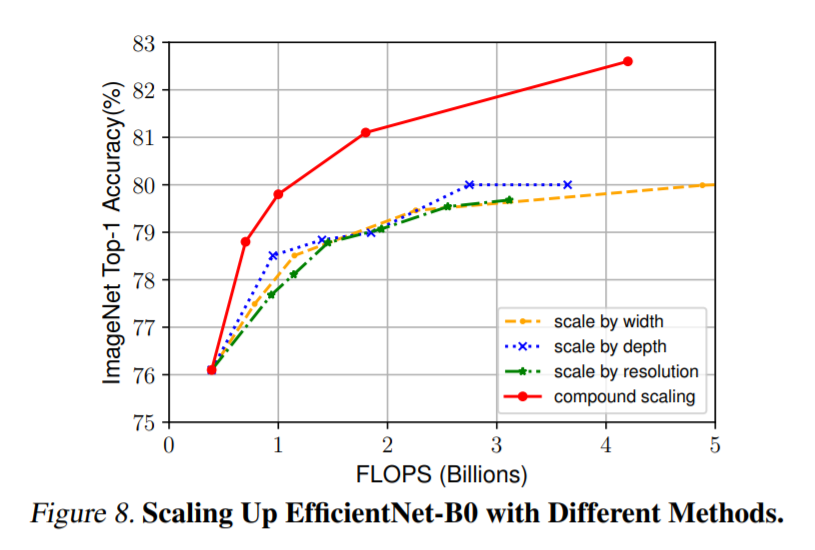
\includegraphics[height=5.0cm]{good_plot.png}
	\end{center}
\end{frame}

\begin{frame}{Пример хорошего графика из жизни}
	\begin{center}
		\fbox{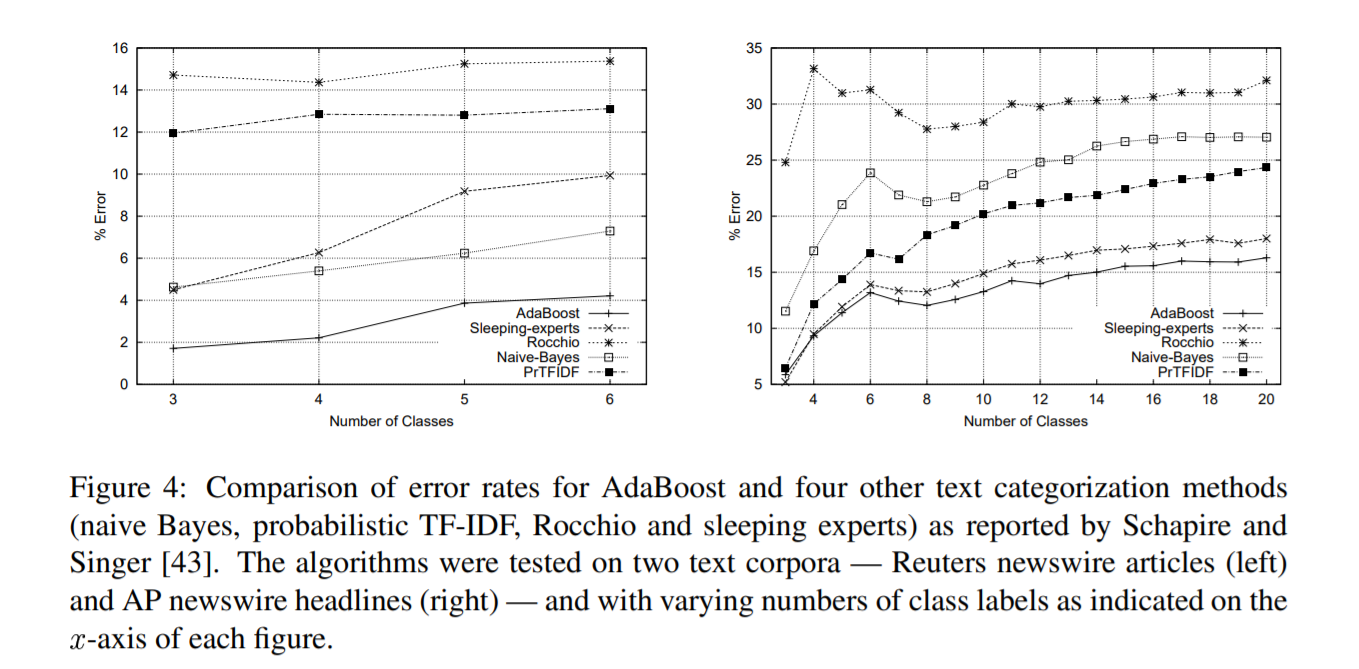
\includegraphics[height=5.0cm]{good_plot_black.png}}
	\end{center}
	Стоит задумываться о том, как будет выглядеть график, если он будет отображаться чёрно-белым.
\end{frame}

\begin{frame}{Думайте об оформлении результатов}
    \begin{center}
        {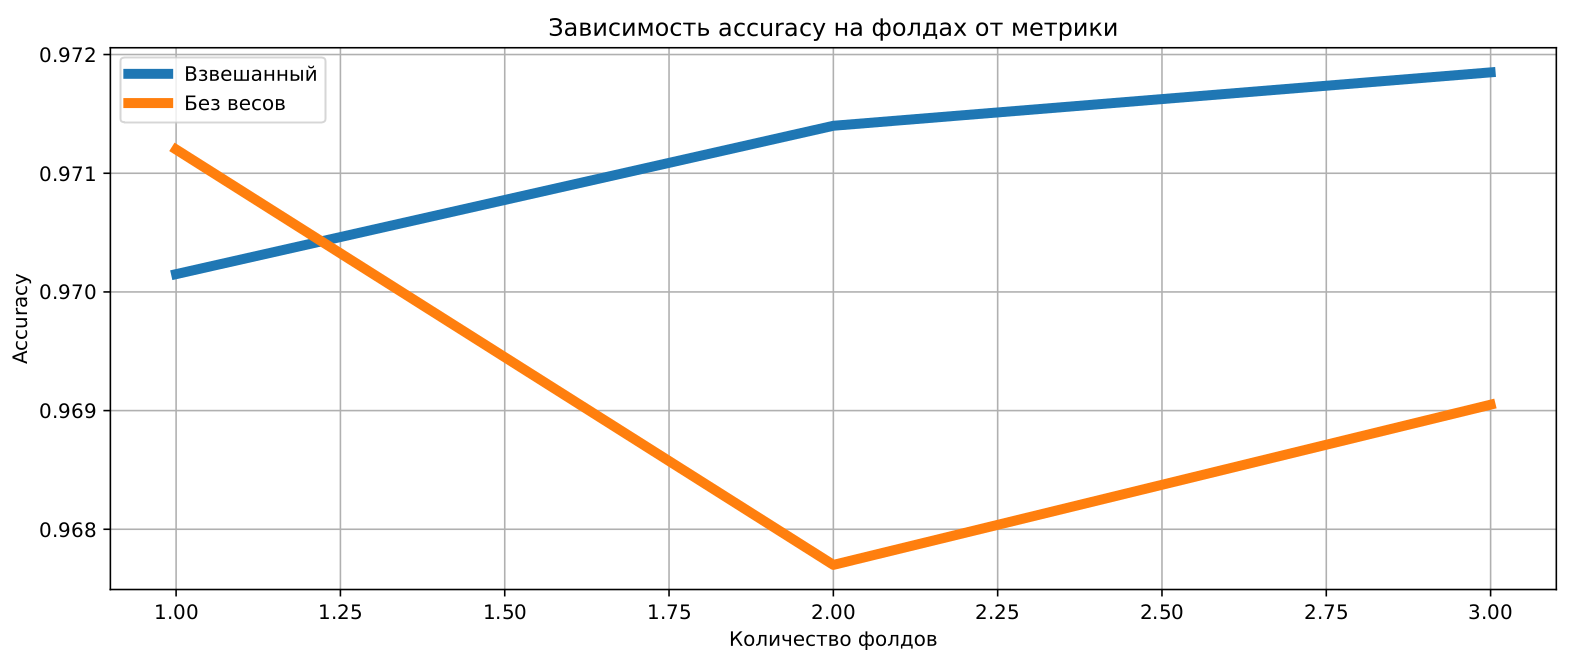
\includegraphics[height=4.8cm]{bad_graphic.png}}
    \end{center}

    \textcolor{red}{Что плохо на этой картинке?}
    \pause{
        \begin{itemize}
            \item Опечатки
            \item Неправильная подпись по оси $x$
            \item Нет отношения порядка на оси $x$
            \item Слишком подробная шкала по оси $x$
        \end{itemize}
    }
    \end{frame}

\end{section}

\begin{section}{Огранизация страниц}

\begin{frame}{Пример плохо организованной страницы}
	\begin{center}
		\fbox{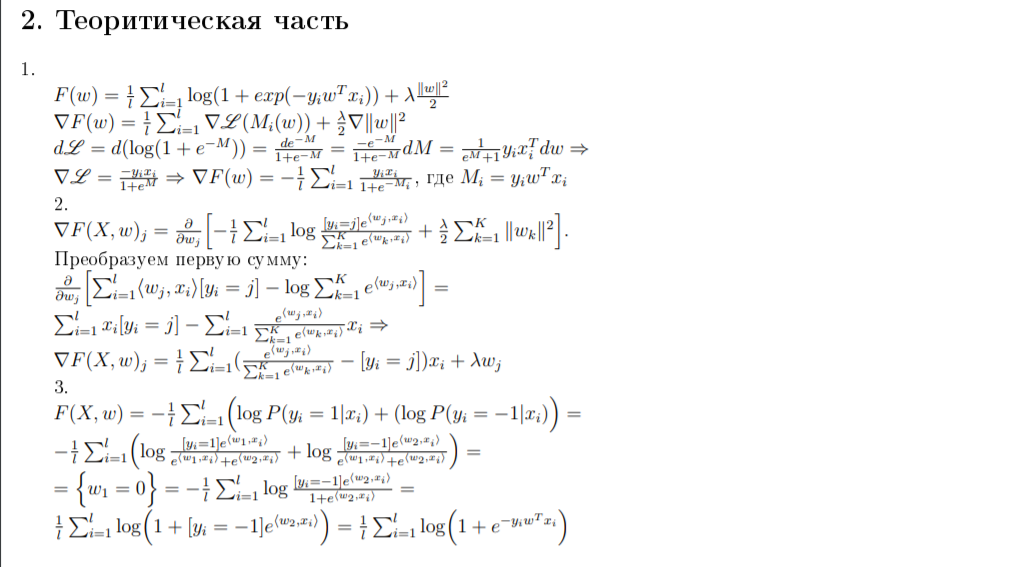
\includegraphics[height=5.0cm]{bad_formating.png}}
	\end{center}
	Формулы <<съехали>> и стали плохо читаться.
\end{frame}

\begin{frame}{Пример плохо организованной страницы}
	\begin{center}
		\fbox{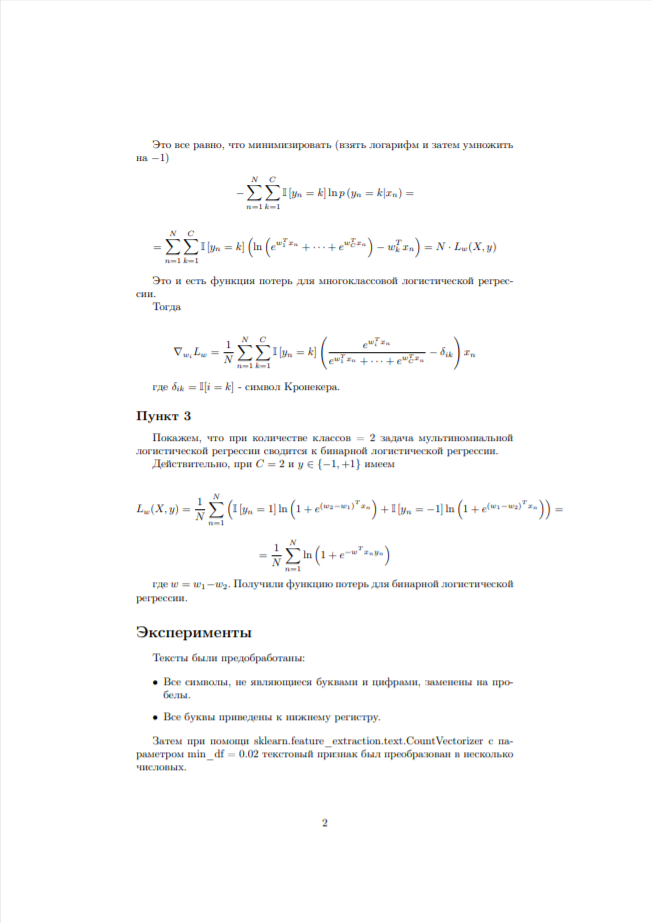
\includegraphics[height=6.5cm]{huge_borders.png}}
	\end{center}
	Слишком большие поля.
\end{frame}

\begin{frame}{Пример плохо организованной страницы}
    \begin{center}
        \fbox{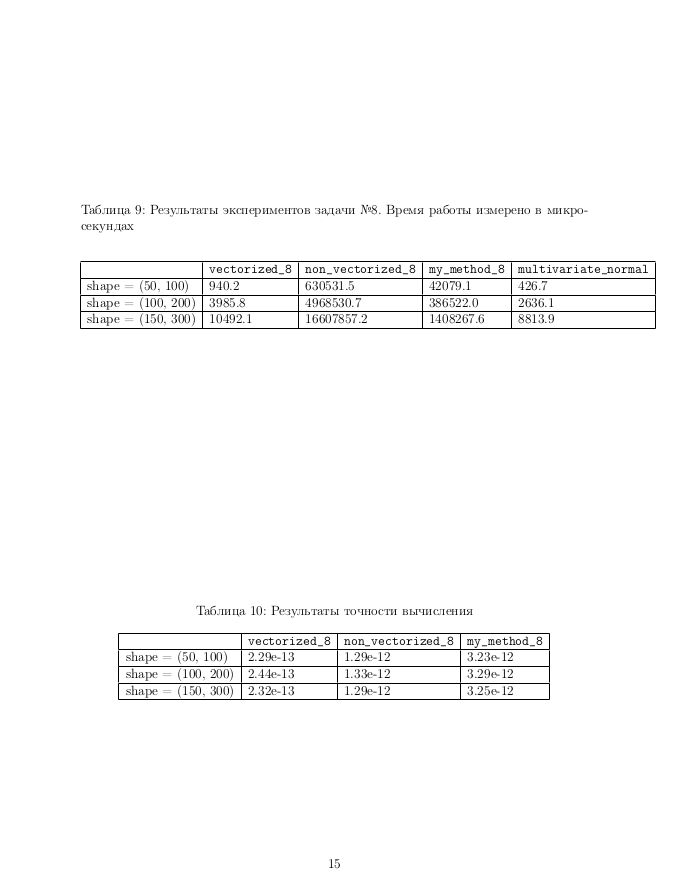
\includegraphics[height=6.5cm]{bad_page.png}}
    \end{center}
    Есть большие пустые пространства на странице.
\end{frame}

\begin{frame}{Пример плохо организованной страницы}
    \begin{center}
        \fbox{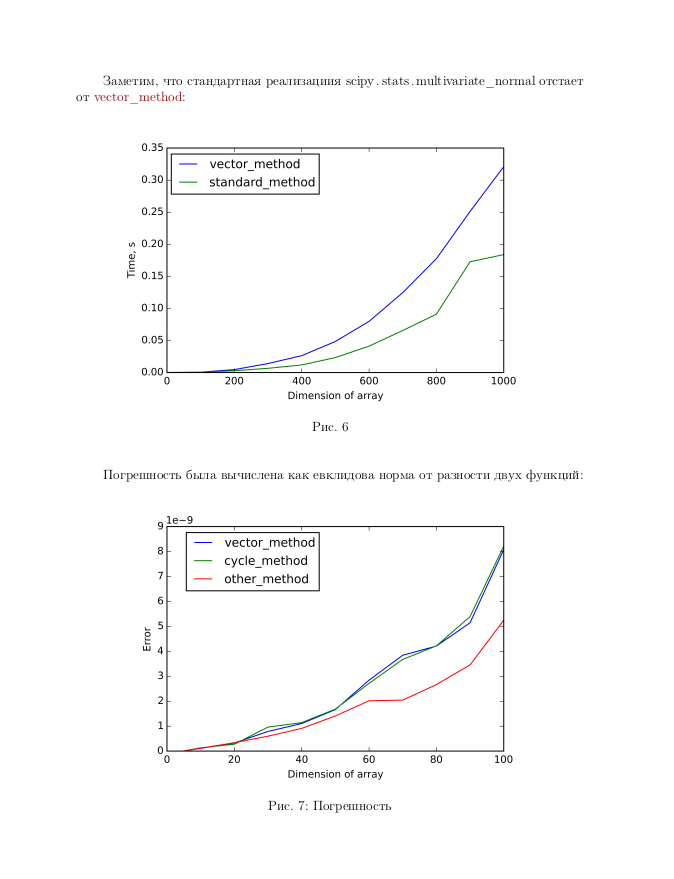
\includegraphics[height=6.5cm]{bad_page2.png}}
    \end{center}
    Графики занимают слишком много места.
\end{frame}

\begin{frame}{Пример плохо организованной страницы}
    \begin{center}
        \fbox{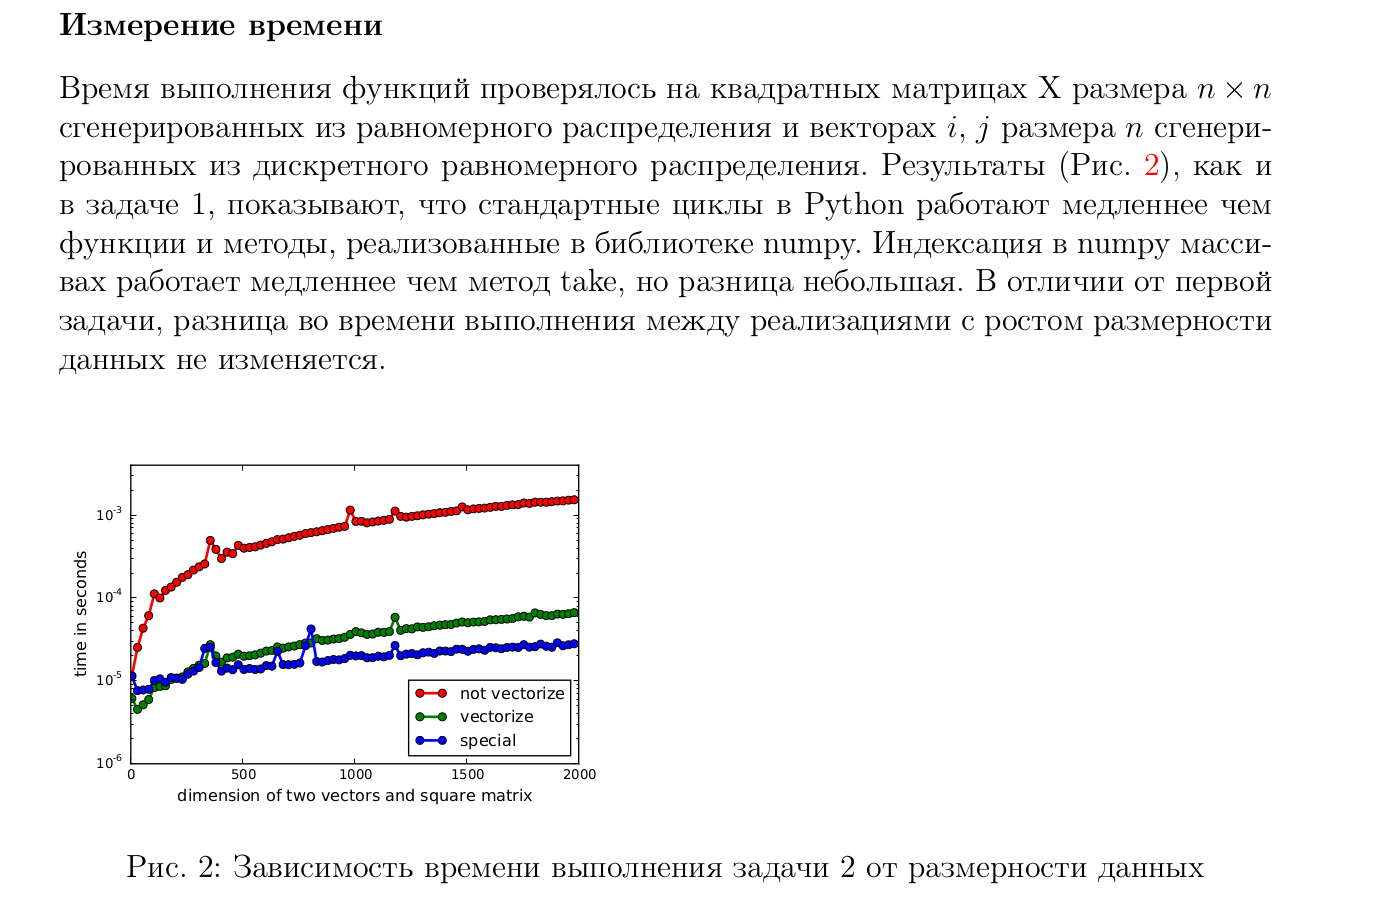
\includegraphics[height=5cm]{bad_page5.png}}
    \end{center}
    Есть большие пустые пространства на странице.
\end{frame}

\begin{frame}{Пример плохо организованной страницы}
    \begin{center}
        \fbox{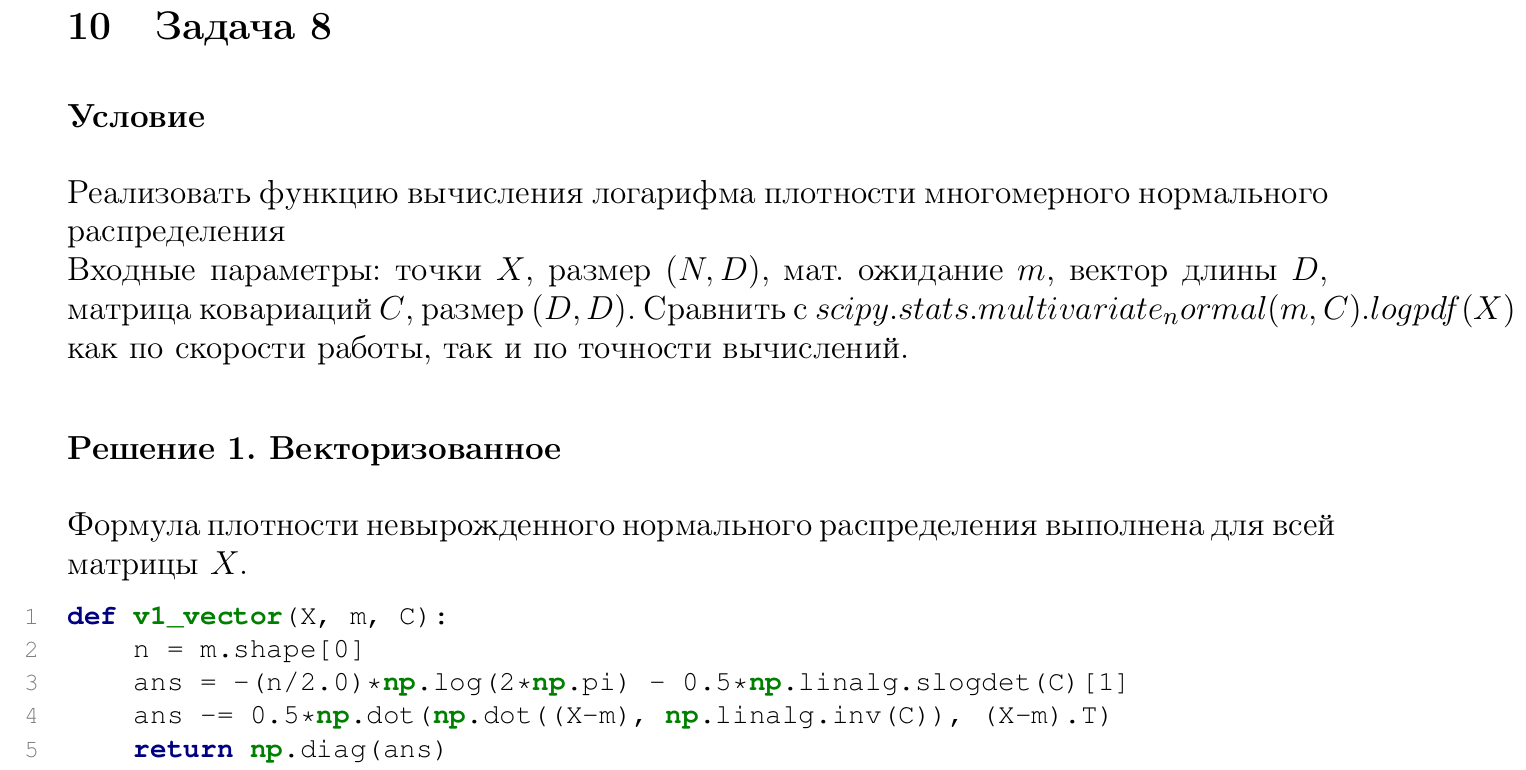
\includegraphics[height=5cm]{bad_page3.png}}
    \end{center}
    Текст залезает на поля страницы.
\end{frame}

\begin{frame}{Примеры хорошо организованных страниц}
	\begin{center}
		\begin{tabular}{ll}
			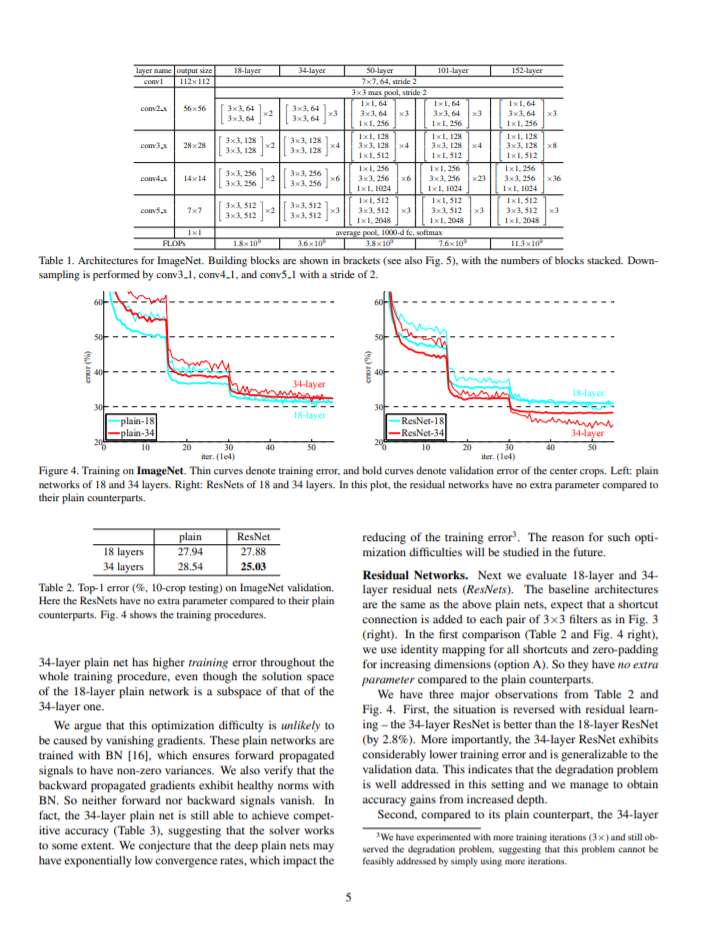
\includegraphics[height=7.5cm]{good_formatting.png} & 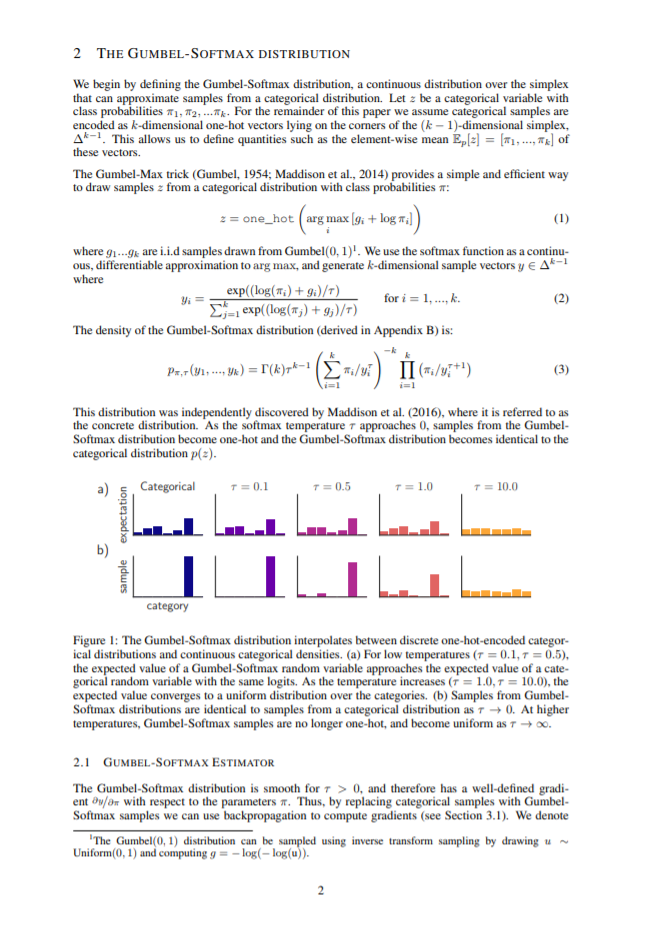
\includegraphics[height=7.5cm]{good_formatting_2.png}
		\end{tabular}
	\end{center}
\end{frame}

\end{section}

\begin{frame}{Все числа указываются с необходимым числом знаков}
    \begin{center}
        {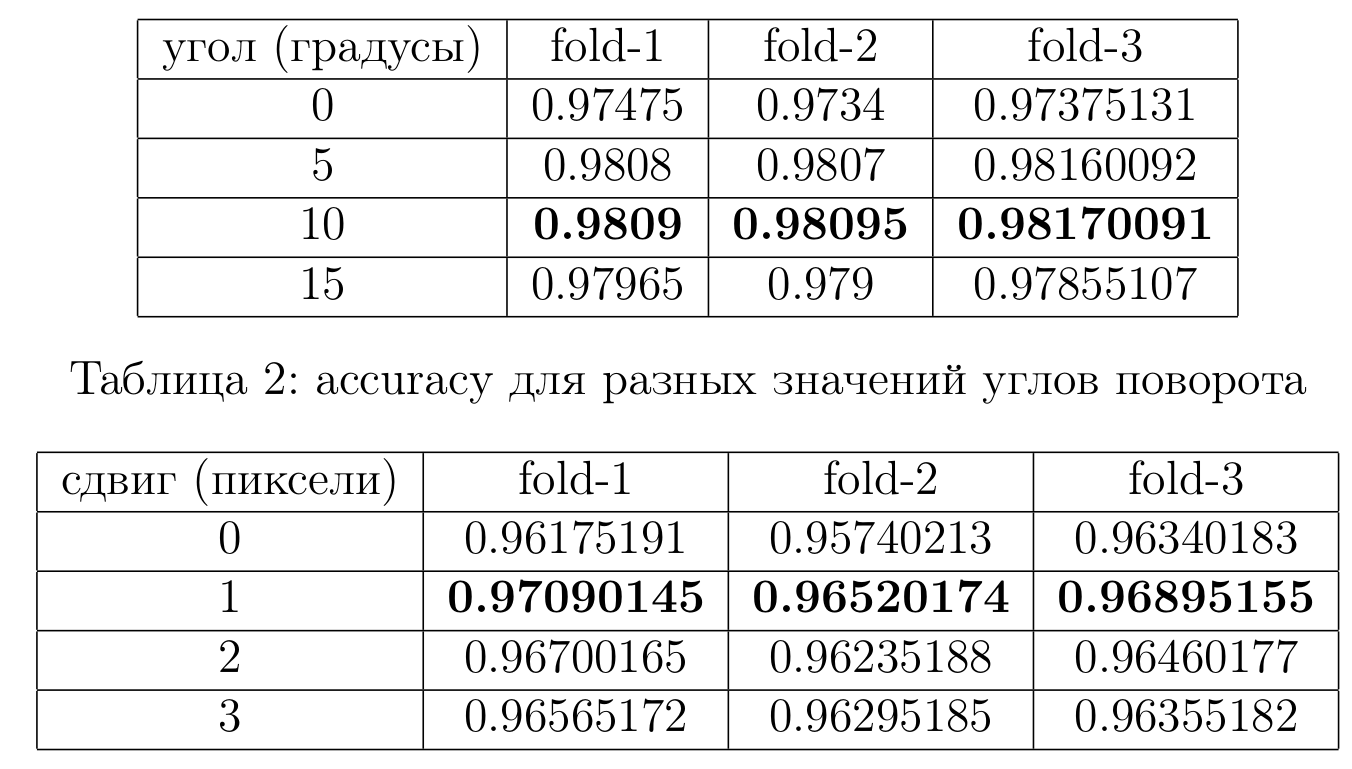
\includegraphics[height=6.5cm]{bad_numbers.png}}
    \end{center}
    Число указывается с точностью до 2 или 3 знака после запятой.
\end{frame}

\begin{frame}{Избегайте длинных предложений}
    Далее в опытах, для настройки нашего метода, подбора оптимальных параметров, нам придётся использовать кросс-валидацию. Но эта операция занимает очень много времени, поэтому так как все стратегии, перечисленные выше, являются точными, то есть одинаково классифицируют один объект, имея одинаковую обучающую выборку, нам нужно измерить время их работы, и определить лучшую стратегию. Результат опыта на ниже приведённом рисунке.
\end{frame}

\begin{frame}{Чего ещё следует избегать?}
\begin{itemize}
    \item Ненаучной лексики (<<результаты модели получились фиговые>>)
    \item Орфографических ошибок (установите проверку в среде)
    \item Грамматических, синтаксических и других ошибок
    \item Повествования от первого лица единственного числа
    \item Обращений к читателю (<<вашему вниманию представлены результаты экспериментов>>)
    \item Смешения стиля использования буквы <<ё>> (либо везде используете <<ё>>, либо везде <<е>>)
\end{itemize}
\end{frame}

\begin{section}{Итог}

\begin{frame}{Итог: элементы хорошего отчёта по заданию}
\begin{itemize}
    \item Отчёт подготовлен в системе \TeX
    \item Объём отчёта: 5--20 страниц
    \item Текст отчёта не повторяет полной формулировки задания
    \item Структура отчёта соответствует пунктам задания
    \item Используются векторные шрифты
    \item Графики оформлены надлежащим образом
    \item Шкала для графиков выбрана правильно
    \item На разных графиках результаты для одинаковых методов отображаются одним и тем же цветом
\end{itemize}
\end{frame}

\begin{frame}{Итог: элементы хорошего отчёта по заданию}
\begin{itemize}
\item Между расположением графиков и местами их упоминания в тексте относительно небольшое расстояние (на той же или на соседней странице)
\item На страницах не должно быть много пустого места
\item В большинстве случаев графики/таблицы/псевдокоды алгоритмов не должны занимать большей части одной страницы отчёта
\item Все числа в тексте/таблицах указаны с необходимым числом значащих цифр
\item В большинстве случае в отчёте не должно быть никакого кода
\item Для всех экспериментов описан выбранный дизайн экспериментов, а также сделаны выводы из полученных результатов
\end{itemize}
\end{frame}

\end{section}

\end{document}
